\documentclass[12pt]{article}
\usepackage{xeCJK}  

\usepackage{charter}
\usepackage{fullpage}
\usepackage[colorlinks=false,unicode]{hyperref}
\usepackage{ifthen}
\usepackage{comment}
\usepackage[title,titletoc]{appendix}
\usepackage{pagecolor}
\usepackage{amsmath}
\usepackage{amsfonts}
%\usepackage[normalem]{ulem}
\usepackage{siunitx}
\usepackage{amsthm}
\sisetup{per=slash, load=abbr}

\usepackage{pgfplots}
\usetikzlibrary{positioning}
\usetikzlibrary{fit}
\usetikzlibrary{snakes}
\usetikzlibrary{shapes.geometric}
\usetikzlibrary{patterns}
\usetikzlibrary{shapes,arrows,chains}
\usepgfplotslibrary{patchplots,colormaps}
\usetikzlibrary{calc}
\usetikzlibrary{positioning, fit}
\usetikzlibrary{backgrounds}
\usetikzlibrary{intersections}

\newcommand{\whitepaper}[1]{\begin{center}\fbox{\parbox{0.95\textwidth}{{\footnotesize
#1}}}\end{center}}

\newcommand{\pcolor}{orange!25}

\usepackage{setspace}
\usepackage{algorithm2e}
\bibliographystyle{ieeetr}

\usepackage{geometry}
\geometry{left=3cm,right=3cm,top=1.6cm,bottom=3cm,headheight=0pt,headsep=1.5em}
\usepackage{fancyhdr}
\pagestyle{fancy}
\chead{
\includegraphics[scale=0.1]{../common/Nebulas.png}}  %在此处插入logo.pdf图片 图片靠左
\lhead{} % 页眉中间位置内容
\rhead{}
%\setlength{\topskip}{1em}

\usepackage{enumerate}
\setcounter{tocdepth}{4}
\setcounter{secnumdepth}{4}


\usepackage{indentfirst}


\setCJKmainfont[BoldFont = STSongti-SC-Bold]{STSongti-SC-Regular}
\setCJKfamilyfont{hei}{SIL-Hei-Med-Jian}		%宋体
\setCJKfamilyfont{song}{SimSun}		%宋体
\setCJKfamilyfont{kai}{Kaiti}		%楷体
\setCJKfamilyfont{fang}{song}	%仿宋
\setCJKfamilyfont{li}{song}			%隶书
\setCJKfamilyfont{you}{Yuanti}		%幼圆

\newcommand{\song}{\CJKfamily{song}}	%宋体
\newcommand{\hei}{\CJKfamily{hei}}	%黑体
\newcommand{\kai}{\CJKfamily{kai}}	%楷体
\newcommand{\fs}{\CJKfamily{fang}}	%仿宋
\newcommand{\li}{\CJKfamily{li}}		%隶书
\newcommand{\you}{\CJKfamily{you}}	%幼圆
\newcommand{\reffig}[1]{图\ref{#1}}
\newcommand{\refsec}[1]{\S \ref{#1}}

\onehalfspacing   % ----------设置1.5倍行距(可能有意义,待调整)

%\parindent=20pt  % -------------------首行缩进大小,英文分段就直接0pt了吧。
\setlength{\parindent}{2.1em}
\setlength{\parskip}{0.3\baselineskip}
\newcommand{\dom}{{\; \texttt{dom}\;}}
\newcommand{\xpcomment}[1]{{\color{blue} #1}}

\setCJKsansfont[BoldFont = STHeitiSC-Medium]{STHeitiSC-Light}


\newtheorem{property}{特征}
%\addbibresource{reference.bib}

\begin{document}
\pagestyle{empty}
\renewcommand{\contentsname}{目录}
\renewcommand{\abstractname}{摘要}
\renewcommand{\refname}{参考文献}
%\renewcommand{\nomname}{术语表(按首字母排序)}
\renewcommand{\figurename}{图}
\renewcommand{\tablename}{表}
\renewcommand{\baselinestretch}{1.5}
\renewcommand{\appendixname}{附录}
\renewcommand{\proofname}{证明}

%\pagecolor{\pcolor}

\begin{titlepage}
  \begin{center}
    \vspace*{5.5cm}
    
\includegraphics[scale=0.4]{../common/Nebulas.png}
    \vspace{0.5cm}


    \textbf{\huge{星云链NAX白皮书}}

    \vspace{0.5cm}
    NextDAO Lab
    \vfill
    2019年8月 \\
    版本号:0.0.1
    \textbf{}
  \end{center}

\end{titlepage}
\setcounter{page}{0}
\tableofcontents
\newpage
\setcounter{page}{1}
\pagestyle{fancy}
\vspace*{0.01cm}
\section{星云理念概述}

\subsection{理念和使命}
2008年10⽉31⽇,中本聪(Satoshi Nakamoto)发布⽐特币⽩⽪书~\cite{whitepaper},从此我们迎来了⼀个有区块链的世界。经过十年的发展,⽐特币践⾏了其作为“⼀个去中⼼化电⼦现⾦系统”的初衷。以太坊[x]更进一步,为区块链世界提供了一个运行具有图灵完备性的代码的能用区块链框架。区块链技术在此之后也取得了空前的发展和繁荣。区块链技术本身不是一个全新的技术创新,而是作为一系列技术的组合(包括密码学,分布式系统,博弈论等)而产生的模式创新。在星云的白皮书[x]中提出了自己的主张和解决方案,并始终坚持致力于践行“让每个人从去中心化的协作中公平受益”作为星云使命,落地场景上以实现The Better DAO[x]为目标。


\subsection{区块链协作}
随着科技的发展,协作场景已经从人与人面对面合作变得更灵活、更自由。区块链技术本质上是一个去中心化、非信任、基于博弈的自治体系,其真正的魅力是在去中心化思想下基于共识机制的开放协作模式。目前区块链的协作仍然存在着以下几个问题:

\begin{itemize}

	\item \textbf{协作角色多样化}

	早期比特币社区只有矿工和持币者,有了以太坊之后出现了开发者、应用使用者等,越来越多的人接触到区块链,不同用户角色的责权利如何分配受到挑战。

	\item \textbf{激励方式单一}

	目前大多数公链的共识激励还是以PoW, PoS为主的专注于挖矿的激励,事实说明单一激励不能应对用户角色的逐渐丰富。

	\item \textbf{公平与正向博弈缺失}

	为社区做出贡献的角色并没有得到对应的激励,使得整个区块链没有呈现出正向博弈的。

\end{itemize}

\subsection{技术愿景}
在践行这个使命和达成目标过程中,星云提出了一些路径,其中包括:星云指数(NR)[x], 开发者激励协议[x], 星云原力(NF)以及星云贡献证明(PoD)等。在过去两年中,由于区块链技术得到了前所未有的发展,商业落地的场景和尝试也层出不穷。星云链在坚持最初的主张和愿景的同时,根据自身优势以及在区块链世界摸索前行的中总结的经验,将会有更多的探索和尝试。

\section{NextDAO}
\subsection{区块链协作}
以太坊ERC20的出现,以区块链智能合约技术为基础,成为了一种新型、快捷、低成本的融资方式,但融资过后的协作和管理问题并没有得到很好的解决。这一直都是区块链重要的发展方向之一,并同时带来了很多问题。

The DAO(Decentralized Autonomous Organization)~\cite{DAO},又叫“去中心化自治组织”一个以公开透明的计算机代码来体现的组织,其受控于股东,并不受中心化组织影响。The DAO发布之后,很快被黑客攻击并盗走价值千万美金价值的以太坊,最终导致以太坊硬分叉。虽然The DAO存在着缺陷,但给后续的工作带来了很多借鉴的作用。

星云链致力于区块链协作的发展,并在此基础上提出了基于区块钱协作的框架范式集合:NextDAO。具体包含:公链协作、治理、去中心化金融(DeFi)等,详细如图\ref{fig:nextdao}所示。NextDAO尝试着解决目前区块链的协作当中存在的几个问题:

\begin{enumerate}[\hspace{1cm}(a)]
  \item 激励方式仍以出块奖励为主
  \item 公平与正向博弈缺失
  \item 协作方式单一
\end{enumerate}

\begin{figure}[htbp]
  \centering
  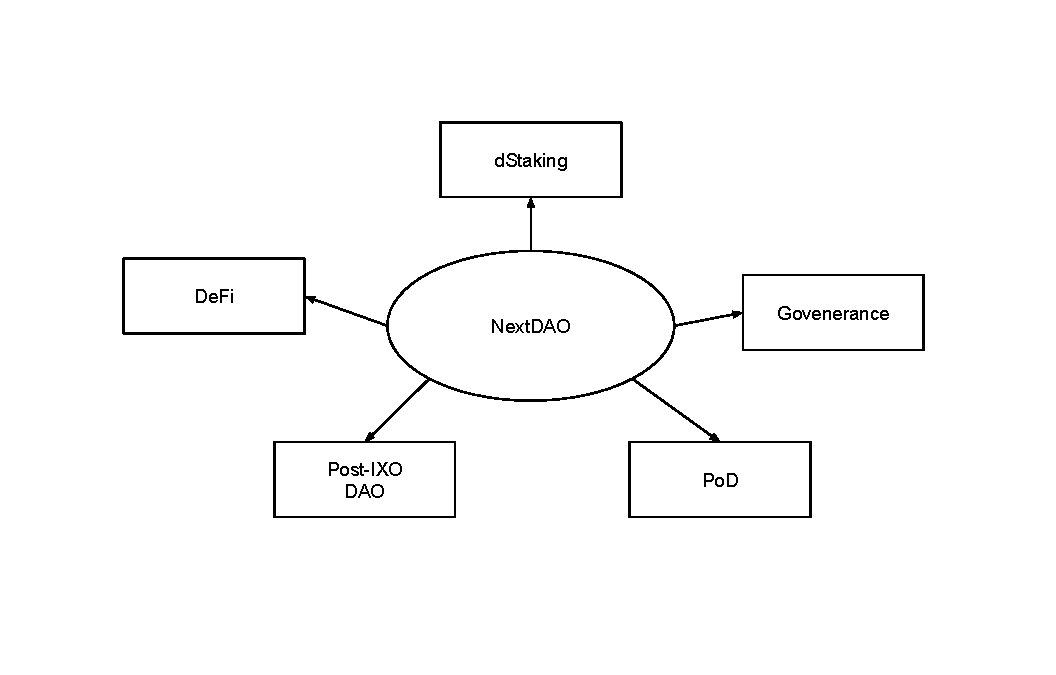
\includegraphics[width=0.5\textwidth]{../common/nextdao.pdf}
  \caption{区块链协作范式集合:NextDAO \label{fig:nextdao}}
\end{figure}

\subsection{公链通证经济}
通证经济(Token Economy),具体表现为包含通证产生、流通、回购、激励等经济模型。通证经济存在于区块链世界各个角落,例如公链生态、DApp应用内部等。公链生态通证经济的典型的案例是以太坊的ERC20,它便利了融资的同时,刺激和繁荣了以太坊生态,也同时带动了整个区块链行业的大发展。因此,公链的价值和创新不仅仅源于在“不可能的三角”上的技术本身的创新,也来源于技术所带来的模式和商业创新。

公链通证经济要考虑的问题是人与人的博弈,需要避免公地悲剧~\cite{TragedyOfTheCommons},通过正向激励促进公链生态的繁荣和发展。大多数公链远达不到以太坊的社区力量,因此以探索区块链应用落地为导向,发展区块链技术,扩大社区共识,才能建立一个适合自身的优秀的公链通证经济,这与发展公链技术创新同等重要。接下来的章节,将详细介绍星云链根据自身的愿景和特点,提出来的基于NextDAO框架的公链通证范式:NAX。

% !TEX root = main.tex
\section{核心系统设计}

\subsection{质押NAS返NAX}
标准:
\begin{enumerate}
\item 四个周期(发行量)调整一次
\item 质押率 == 算力
\item 算力会影响难度
\item 衰减速率
\end{enumerate}

示例:
\begin{enumerate}[a.]

\item 一年减半(2,500,000), 周期:100,000 (两周多)衰减一次\\
衰减系数:0.973\\
math.pow(0.973, 25) = 50\%

\item 一年减半(2,500,000), 周期:50,000 (一周多)衰减一次\\
衰减系数:0.986\\
math.pow(0.986, 50) = 49.4\%

\item 两年减半(5,000,000), 周期:100,000 (两周多)衰减一次\\
衰减系数:0.986\\
math.pow(0.986, 50) = 49.4\%

\item 两年减半(5,000,000), 周期:50,000 (一周多)衰减一次\\
衰减系数:0.993\\
math.pow(0.993, 100) = 49.5\%

\end{enumerate}

新提议(质押消耗NAS) -- 感觉不是特别友好

如果我们需要维护一个质押率,达到一定的博弈平衡,可以添加,根据质押数量,消耗NAS的质押场景,也就是说,当质押分配到的NAX不合算的时候,用户可能会取消质押。当质押数变小的话,又会使得质押所得的NAX变得更多,所以又有人开始质押。

质押消耗的NAS可以被看作是BTC挖矿中消耗的电费。

收集的消耗的NAS会收集成为社区建设基金:Go Nebulas

公式如下:其中

        第\(i\)期用户\(j\)获得的NAX: \(K_{i,j}\)

        第\(i\)期用户\(j\)的质押量: \(P_{i,j}\)

        第\(i\)期用户\(j\)的质押时间: \(T_{i,j}\)

        第\(i\)期初始总增发量:\(C_i\)

        第\(i\)期增发比例: \(\lambda_i\)

        衰减系数:\(B\)

        h是质押高度总和,v是质押数量

\begin{equation}
  K_{i,j} = \frac{P_{i,j} T_{i,j}}{\sum_j P_{i,j} T_{i,j}} \lambda_i C_i
\end{equation}
\begin{equation}
  \lambda_i = f(\sum_j P_{i,j} T_{i,j})
\end{equation}
\begin{equation}
  C_i = C_0 B^i
\end{equation}

\subsection{质押返率\(\lambda\)}
\begin{enumerate}[a.]
  \item 时间。难度问题。早期质押, \(\lambda\)更高,正向量
  \item 预期?质押高度为质数, \(\lambda\)更高 x
  \item 运营活动。。。返回会越来越多?上一高度交易量越高, 此高度 \(\lambda\)更高 x
  \item 质押率(算力)越高, \(\lambda\)越高,质押率下降,难度下降,收益上升。质押率上升,难度上升。
\end{enumerate}

\begin{equation}
\lambda = (f(a, c, d) + g(h) b) / h
\end{equation}

\subsection{增发周期设定}
可以每100000高度分发一次,也就是高度满足以下性质:

H = h mod 100000 == 0

\subsection{取回质押策略}
满足性质:v越高,取回周期t越长,滞后返还, B是基本量级

B(v) =  floor(sqrt(v) - B) * t

\subsection{系统手续费}
每次增发的时候,新增发所得的4\% 转入NAX的专属项目基金。

矿工费?

固定手续费。发行费。铸币税。

项目团队的预期收益。



NAT的发行是根据每个用户的星云指数、投票行为以及质押情况决定的,没有预发行。

\subsection{概述}
NAT的发行按照星云指数的计算周期进行(注意,投票周期和星云指数周期相同),也就是说,在每个星云指数的计算周期结束,根据该星云指数计算周期每个用户的星云指数情况及投票、质押行为进行发放。
基本来说,
对于周期$i$,系统中新增的NAT $\mathcal{T}_i$分为三个部分:根据地址的星云指数获得的部分$\mathcal{A}_i$、投票激励部分$\mathcal{V}_i$、质押激励部分$\mathcal{D}_i$。
另外,用户用于投票的NAT会被销毁一定的比例,假设对于周期$i$,系统中因投票减少的NAT为$\mathcal{M}_i$,则系统中总的NAT发行量为:
\begin{align}
\sum_{i=1}^{\infty} (\mathcal{A}_i + \mathcal{V}_i + \mathcal{D}_i - \mathcal{M}_i)
\end{align}

为方便说明,此处先给出本章涉及到的符号,并给出相应的说明,
\begin{itemize}
\item $\mathcal{C}_i$:系统在周期$i$的星云指数总和;
\item $c_{i,j}$:用户$j \in \mathcal{U}$在周期$i$的星云指数值;
\item $d_{i,j}$:用户$j \in \mathcal{U}$在周期$i$质押的NAS总量;
\item $v_{i,j}$:用户$j \in \mathcal{U}$在周期$i$投票的NAT总量。
\end{itemize}

\subsection{根据地址的星云指数获得的部分}
此部分与用户的星云指数相关,定义为:
\begin{align}
    f(x) = g(x)\lambda^i
\end{align}
\noindent 其中$x$为用户星云指数;$g(x)$为调整NAT总量与星云指数总量关系的比例函数,且满足$g(0) = 0$;$\lambda$为衰减系数,且$\lambda < 1$。
由于$\lambda < 1$,易知$\lim_{i\to \infty}f(x) = 0$。

可知,此部分在周期$i$的新增总量为:
\begin{align}
\mathcal{A}_i = \sum_{i=1}^{\infty}f(\mathcal{C}_i)。
\end{align}

\subsection{投票激励部分}
投票激励部分和用户的投票行为,以及星云指数相关,对于用户$j \in \mathcal{U}$,投票激励为:
\begin{align}
\mu f(x_{i-1,j}) \min\{\frac{v_{i,j}}{f(x_{i-1,j})},1\}
\end{align}
\noindent 其中$\mu$为投票激励系数,$\mu > 1$,表示对用户的投票行为给予额外的奖励,可以根据系统中流通的NAS的数量变化调整。

\subsection{质押部分}
质押部分获得的NAT应与部分NAS提升星云指数获得的部分存在相关性。根据星云指数的性质可知,给定NAS,其存在星云指数的上限$h(d_{i,j})$~\cite{ImproveNR},

则定义质押部分获得的NAT为:
\begin{align}
\mathcal{D}_i = \sum_{i=1}^{\infty}\alpha f(h(d_{i,j}))
\end{align}
\noindent 其中$\alpha$为质押激励系数。


\subsection{销毁部分}
\label{burn}
用户每次投票,都会有一部分被销毁,剩余的部分返还给用户,同时,NAT项目团队为了支付投票活动的必要开销,对每笔投票征收$\theta\%$的费用。因此,对每个用户而言,定义销毁部分为:
\begin{align}
(1-\theta\%) \times \beta^i \times v_{i,j}
\end{align}
\noindent 其中,$\beta$为销毁系数,且$\beta < 1$。因此,
\begin{align}
    \mathcal{M}_i = \sum_{i=1}^{\infty} (1-\theta\%) \times \beta^i \times v_{i,j} 。
\end{align}

\subsection{分析}

注意:
\begin{itemize}
\item 目前版本暂定赞同票与反对票没有区别,即返还比例相同。之后可根据票种设定并乘上不同的返回参数$\mu_1$;
\item 若考虑到投票完成后系统的总星云指数变化,则可再乘上一个系数$\mu_2$,用于反应该周期系统的繁荣度。
\end{itemize}


\begin{property}
本算法能满足NAT总量的收敛性,即NAT总量在任何时候都不会超过一个上限。
\end{property}
\begin{proof}
	根据《星云技术白皮书》的设定,NAS的固定总量为$10^9$,平均每周大约增发(在固定总量的基础上)$0.2\%$,故在第$n$个投票周期市面上现存NAS总量不会超过$10^9(1+0.002n)$。
	
	接下来我们证明所有地址一个周期内的资产中值(见《星云指数黄皮书》中的定义)总和不会超过市面上现存NAS总量。这是因为,对于任意一笔数量为$y$的NAS资产,他只能最多在一个地址内存在该周期一半以上的时间(三天半),故最多给全网节点的总资产中值提供$y$的贡献。
	
	同样根据星云指数黄皮书的设定,任何一个地址的星云指数值不会超过该地址的资产中值(指同样一个周期内,注意星云指数和NAT的计算都是以周为单位,具有同步性),这是因为黄皮书星云指数计算公式$\Omega(\cdot)\Psi(\cdot)$中,以资产中值为输入的Wilbur函数$\Omega(\cdot)$满足$\Omega(x)\leq x$,且出入度函数$\Psi(\cdot)$值域不超过1。
	
	结合上述结论,可得在第$n$个周期,所有地址星云指数总和不超过$10^9(1+0.002n)$,从而根据地址星云指数获得的NAT不超过$g(10^9(1+0.002n))\lambda^n$。
	
	又因为投票激励部分的NAT不超过增发部分乘以$\mu$,故即使加上返还部分带来的增量,周期$n$内激励部分NAT的总增量不超过$\mu g(10^9(1+0.002n))\lambda^n$。另外,质押部分带来的增量不超过NAS总量$g(10^9(1+0.002n))\lambda^n$。
	
	最后,欲证NAT总量的收敛性,因为根据地址的星云指数获得的部分、质押部分和激励部分均随时间指数级衰减,故只需证明级数:
	\begin{align}
	\sum_{n=1}^{\infty} \mu g(10^9(1+0.002n))\lambda^n
	\end{align}
	收敛。由于$g(\cdot)$为线性函数,故
	\begin{align}
	\lim_{n\rightarrow \infty} \frac{\mu g(10^9(1+0.002(n+1)))\lambda^{n+1}}{\mu g(10^9(1+0.002n))\lambda^n} = \lambda <1
	\end{align}
	由比式判别法可得该级数收敛,证毕。
\end{proof}
同时,上述投票算法具有下列良好性质。
\begin{enumerate}
	\item \textbf{抗滚雪球效应:} 如若简单的按固定比例返还NAT,则一个用户可以每次投出所有的NAT并享受大于1比例的返还(如1.1),则其总NAT将按$1.1^n$指数级上升,增长过于庞大。
	\item \textbf{抗收买性:} 若一个低星云指数的用户以购买的方式获取大量NAT并用于投票,由于对低星云指数用户我们设定的对应$x_{i-1}^j$较低,返还的NAT很少,大部分都被烧毁,导致该用户剩余NAT很少作为惩罚。
	\item \textbf{抗通货膨胀:} 由于系统增发NAT比例与当前市场NAT总量有关,可有效控制NAT的贬值。
	\item \textbf{头部效应:} 早期拥有高星云指数的用户能拥有更高NAT总量。
\end{enumerate}

\section{应用场景展望}
为了尊重资产的公平性,正当性,确权性,我们把分发模型的设计简洁、明了、有效。结合星云的生态特点,将更多的激励和博弈场景交给了应用场景本身,应用场景中的激励和消耗场景可以更加变化、多样。在本章节中,我们针对星云中已经存在的或是未来的应用场景进行一些展望,如图\ref{fig:nax_ecosys}所示,我们可以比较清晰的勾勒出NAX在星云生态的正向激励作用。

\begin{figure}[h]
  \centering
  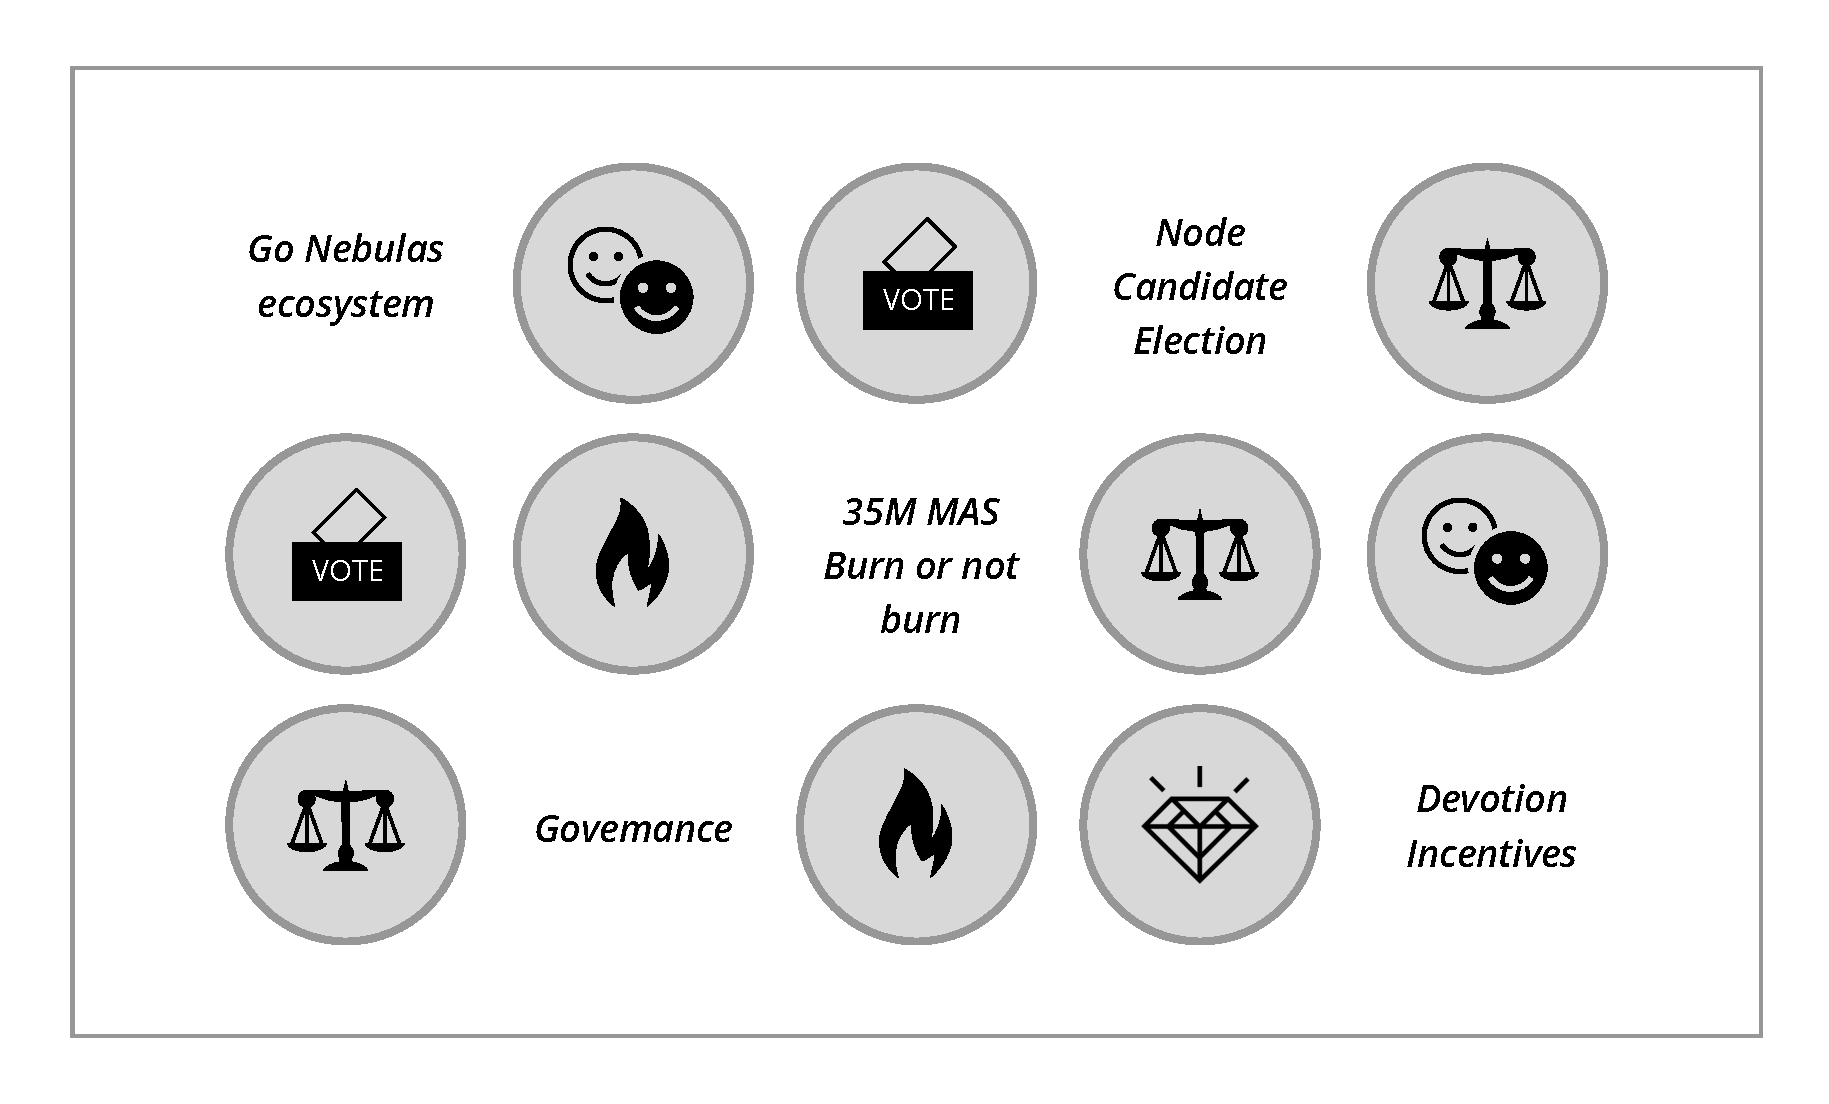
\includegraphics[width=0.6\textwidth]{../common/usecases.pdf}
  \caption{NAX在星云生态中的使用场景 \label{fig:nax_ecosys}}
\end{figure}

\subsection{生态贡献激励}
在白皮书中,从贡献证明的共识算法(PoD, Proof of Devotion),到星云的愿景的提出:在去中心化的协作中公平受益,再到2019年初,Go Nebulas平台的上线,都始终贯穿着星云对生态贡献度衡量的探索。这些都是星云进一步朝着Autonomous Metanet目标前进的重要环节。为此提出一种以质押投资基金为权益证明的激励方式,使之运用到不同场景的激励当中。具体的操作是,将项目投资基金(通常以NAS形式存在)进行质押,这部分资金质押所得的NAX权益,将作为该生态场景的NAX激励权益基金。

\subsubsection{Go Nebulas激励}
星云基金会将会投入不少于$3,000,000$NAS资金,用于资助Go Nebulas平台上的项目,而且根据需求,基金会还将随时追加资金的投入。这部分资金可以投入到质押当中,产生的权益将用来激励在Go Nebulas平台上做出不同贡献的权益证明,即在获得NAS资金作为报酬之外,还将获得由Go Nebulas平台制定的规则下的NAX激励,作为对星云生态做出贡献的权益,可以在星云生态上行使相应的权益和治理。详细的激励方案将由Go Nebulas的运营团队管理者或社区的参与者共同制定。激励可以分为以下几类:

\begin{enumerate}[\hspace{1cm}(a)]
  \item 核心基础建设
  \item 市场拓展
  \item 推广与邀新
  \item 提案与参与
\end{enumerate}

Go Nebulas平台除了是一个投入社区建设,获得NAX激励的重要方式之外,也同样是一个NAX的重要使用场景,消耗场景包含(不局限)于以下几类:
\begin{enumerate}[\hspace{1cm}(a)]
  \item 创建和发起提案
  \item 提案通过与否决
  \item 项目进行中的质押
\end{enumerate}

\subsubsection{基金会核心成员激励}
成为基金会核心团队的成员,包括兼职的人员,在获得相应的工资作为报酬之外,也将获得由基金会质押所产生的NAX权益作为额外的贡献证明。

\subsection{PoD共识探索}
随着星云对PoD研发的推进,去中心化是星云链的必由之路,NAX将可能在PoD中扮演重要角色,有效地结合主网正在研发的PoD技术创新成为新型共识算法的基础和方向。上一节讨论了NAX在生态中的激励场景, 加上NAX的单一的质押的发行方式,获得NAX的方式只能通过以下方式获得:
\begin{enumerate}[\hspace{1cm}(i)]
  \item 贡献资产的流动性
  \item 投入星云链建设
  \item 参与社区治理场景
\end{enumerate}

从另一外角度不难得出,NAX可以被看作为星云生态的贡献凭证。PoD顾名思义是贡献度证明,区别于PoW、PoS的本质在于,星云链更看中区块链协作当中,以不同角色对生态的贡献作为出块奖励的依据,而不仅依赖算力的大小或是筹码多寡。

在选择共识委员会的时候,可以引入NAX的权益多少来影响出块的概率大小。共识节点委员会的产生,无论是链下还是链上产生,NAX也将可以成为投票的重要依据。现在先链下节点竞选为例,阐述说明节点可能的方式,最终的形式将以官方发布的PoD技术文档为准:

\begin{enumerate}[\hspace{1cm}(a)]
  \item 节点委员会成员由NAX投票选出来
  \item 需要销毁相应量的NAX,并质押NAS
  \item 节点将分多个赛道,丰富生态多样性
  \item 主网PoD共识算法将引入NAX作为参数影响出块权益的分配
\end{enumerate}

\subsection{链上治理场景}
在星云生态的发展进程中,会出现各种各样的评选、选举等活动。为了提高社区生态中的参与度,每个活动将根据需要,使用NAX作为权益证明介质将会在投票和激励策略中发挥重要角色。

例如接下来关于如何处理社区预留的$35,000,000NAS$的方案,将成为比较早期的由社区来贡献方案,并由社区来投票决定处理方案的活动案例。星云基金会曾提议销毁,其中一种可能的方案是,每个月发起一次使用NAX的投票销毁社区预留剩余NAS总量的 \(\lambda\) \% , \(\lambda\) \% 是当前NAS质押率占流通总量的份额,我们也鼓励社区提供更加有效、积极的方案,共同决定这部分资产的使用。

\subsection{星云生态推广}
星云基金会扶持开发的,基础生态产品是星云链生态使用的重要入口,这里包含现在的,还有将来基金会孵化的星云生态产品,例如:NAS nano Pro~\cite{NASnano} 、Explorer~\cite{explorer}和Nebulas DEX等。随着NextDAO的推进以及社区治理的前进,社区里将会出现越来越多的NRC20 Token和治理尝试。这些币种有对生态工具的强烈需求,例如:NAS nano Pro和Explorer等。资源空间有限的情况下,为了使得星云生态相关的产品推出更多优秀好的项目,将可能会使用NAX作为平台征选优秀项目的工具以及保证金,这些保证金也同样可以作为生态项目的活动和激励经费,用于投入到平台的建设当中。

\section{Conclusion}
In order to better realize the concept, vision and align with the characteristics of Nebulas' own ecosystem, Nebulas proposes a economy that adapts to its own philosophy and development. Throughout this document, we analyzed the fairness, legitimacy, power, and motivation of NAX throughout Nebulas' philosophy, ecology, development, collaboration, and governance. This is a demonstration and a beginning of NextDAO's direction. During the process, more unique and valuable ideas will emerge and as such, we expect the community to join in enriching the content and utilization of NextDAO.

%\printbibliography
\newpage
\bibliography{reference}

\newpage 
\begin{appendices}
\section{NAX分析}
由于每期增发池中未发放的部分滚入下一期增发池中,因此总发行量为固定值
\begin{equation}
  \sum_{i,j} K_{i,j} = \sum_i C_0 \mu^i = \frac{C_0}{1-\mu}
  \end{equation}
  令此上界为100亿(\(10^{10}\)),可解出\(C_0 = 10^{10}(1-\mu) = 1.9\times10^7\)。

\subsection{发行量分析}


\subsection{反作弊分析}

%\section{Nebulas Asset Supervision}

\label{supervision}

As show in Figure~\ref{fig:assets}, Nebulas assets include two parts: Community public assets and Nebulas Foundation assets.

\subsection{Community public assets}

\subsubsection{Composition}

\begin{itemize}
	\item 35,000,000 NAS (35\% of total circulation): community reserved assets as stated in the \textit{Nebulas Non-technical Whitepaper}
    \item 8,219.1744 NAS/Day: from consensus/block generation issuance, includes:
	    \begin{itemize}
			\item 2\%: Consensus/block generation issuance
			\item 1\%: Nebulas Council Project Development Fund reserve
		\end{itemize}
	\item 1\%(initial): Native incentive for Developer Incentive Protocol (DIP)~\cite{mauvepaper}, since May 13, 2019
\end{itemize}

\subsubsection{Supervision}

Public assets belong to the Nebulas community; they are automatically distributed and managed via the on-chain governance process and is overseen by the Nebulas Council.

\subsection{Nebulas Foundation assets}

\subsubsection{Composition}

\begin{itemize}
	\item 20,000,000 NAS (20\%): Nebulas team reserved as stated in the \textit{Nebulas Non-technical Whitepaper}
    \item 5,000,000 NAS (5\%): Nebulas Community Development Fund (Eco-investment Balance)
	\item Early private equity project development funds
	\item Early ecological investment income
\end{itemize}

\subsubsection{Supervision}

The Nebulas Foundation assets are managed by the Nebulas Foundation. The Foundation shall ensure that the use of asset information is open and transparent.

\begin{figure}
	\centering
	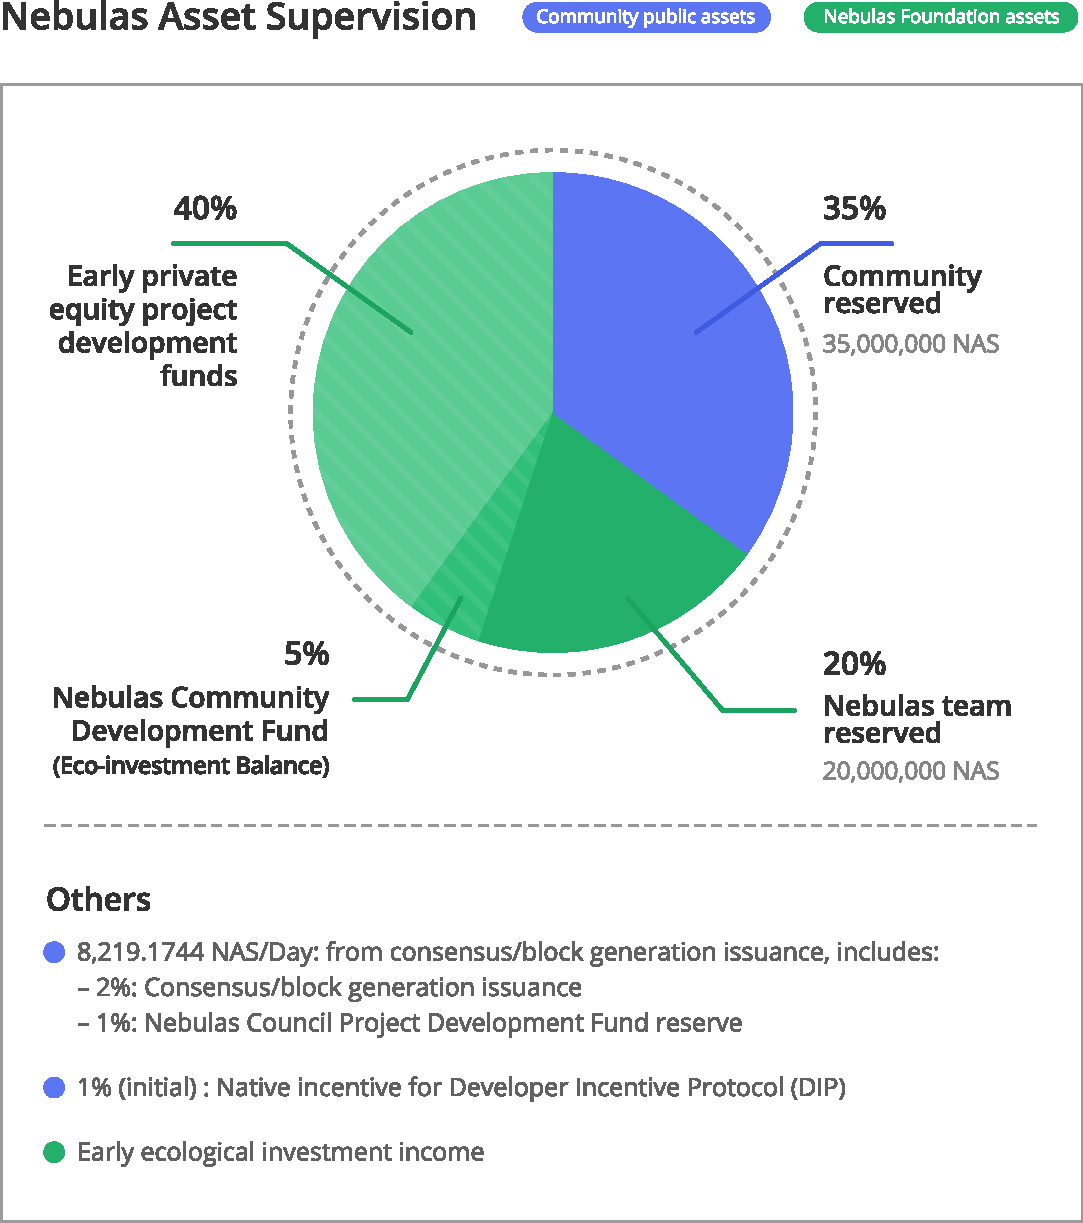
\includegraphics[width=1\textwidth]{../common/en/assets.pdf}
	\caption{Nebulas Assets Supervision \label{fig:assets}}
\end{figure}
\section{Change Log}
\begin{itemize}
\item{0.0.1} Release. 2019.8
\item{0.0.2} Release. 2019.11
\end{itemize}

\end{appendices}
\end{document}
